\documentclass{article}

\usepackage{color}
\usepackage{listings}
\usepackage{fullpage}
\usepackage{graphicx}
\usepackage{hyperref}

\definecolor{gray_ulisses}{gray}{0.55}
\definecolor{castanho_ulisses}{rgb}{0.71,0.33,0.14}
\definecolor{preto_ulisses}{rgb}{0.41,0.20,0.04}
\definecolor{green_ulises}{rgb}{0.2,0.75,0}

\lstdefinelanguage{HaskellUlisses}
{
	basicstyle=\ttfamily\scriptsize,
	%backgroundcolor=\color{yellow},
	%frameshape={RYRYNYYYY}{yny}{yny}{RYRYNYYYY}, %contornos... muito nice...
	sensitive=true,
	morecomment=[l][\color{gray_ulisses}\scriptsize]{--},
	morecomment=[s][\color{gray_ulisses}\scriptsize]{\{-}{-\}},
	morestring=[b]",
	stringstyle=\color{red},
	showstringspaces=false,
	numbers=none,
	firstnumber=\thelstnumber,
	numberstyle=\tiny,
	numberblanklines=true,
	showspaces=false,
	showtabs=false,
	xleftmargin=15pt,
	xrightmargin=-20pt,
	emph=
	{[1]
		FilePath,IOError,abs,acos,acosh,all,and,any,appendFile,approxRational,asTypeOf,asin,
		asinh,atan,atan2,atanh,basicIORun,break,catch,ceiling,chr,compare,concat,concatMap,
		const,cos,cosh,curry,cycle,decodeFloat,denominator,digitToInt,div,divMod,drop,
		dropWhile,either,elem,encodeFloat,enumFrom,enumFromThen,enumFromThenTo,enumFromTo,
		error,even,exp,exponent,fail,filter,flip,floatDigits,floatRadix,floatRange,floor,
		fmap,foldl,foldl1,foldr,foldr1,fromDouble,fromEnum,fromInt,fromInteger,fromIntegral,
		fromRational,fst,gcd,getChar,getContents,getLine,head,id,inRange,index,init,intToDigit,
		interact,ioError,isAlpha,isAlphaNum,isAscii,isControl,isDenormalized,isDigit,isHexDigit,
		isIEEE,isInfinite,isLower,isNaN,isNegativeZero,isOctDigit,isPrint,isSpace,isUpper,iterate,
		last,lcm,length,lex,lexDigits,lexLitChar,lines,log,logBase,lookup,map,mapM,mapM_,max,
		maxBound,maximum,maybe,min,minBound,minimum,mod,negate,not,notElem,null,numerator,odd,
		or,ord,otherwise,pi,pred,primExitWith,print,product,properFraction,putChar,putStr,putStrLn,quot,
		quotRem,range,rangeSize,read,readDec,readFile,readFloat,readHex,readIO,readInt,readList,readLitChar,
		readLn,readOct,readParen,readSigned,reads,readsPrec,realToFrac,recip,rem,repeat,replicate,return,
		reverse,round,scaleFloat,scanl,scanl1,scanr,scanr1,seq,sequence,sequence_,show,showChar,showInt,
		showList,showLitChar,showParen,showSigned,showString,shows,showsPrec,significand,signum,sin,
		sinh,snd,span,splitAt,sqrt,subtract,succ,sum,tail,take,takeWhile,tan,tanh,threadToIOResult,toEnum,
		toInt,toInteger,toLower,toRational,toUpper,truncate,uncurry,undefined,unlines,until,unwords,unzip,
		unzip3,userError,words,writeFile,zip,zip3,zipWith,zipWith3,Impl,Equiv,Prop,Neg,Cnj,Dsj
	},
	emphstyle={[1]\color{blue}},
	emph=
	{[2]
		Bool,Char,Double,Either,Float,IO,Integer,Int,Maybe,Ordering,Rational,Ratio,ReadS,ShowS,String,NoTriangle,Equilateral,Rectangular,Isosceles,Other,Shape
	},
	emphstyle={[2]\color{castanho_ulisses}},
	emph=
	{[3]
		case,class,data,deriving,do,else,if,import,in,infixl,infixr,instance,let,
		module,of,primitive,then,type,where
	},
	emphstyle={[3]\color{preto_ulisses}\textbf},
	emph=
	{[4]
		quot,rem,div,mod,elem,notElem,seq
	},
	emphstyle={[4]\color{castanho_ulisses}\textbf},
	emph=
	{[5]
		EQ,False,GT,Just,LT,Left,Nothing,Right,True,Show,Eq,Ord,Num
	},
	emphstyle={[5]\color{preto_ulisses}\textbf}
}

\lstnewenvironment{code}
{\lstset{language=HaskellUlisses}}
{\smallskip}


\begin{document}
\setlength{\parindent}{0cm}
\title{Software Testing Assignment 6}
\author{Cindy Berghuizen, Omar Pakker, Chiel Peter,  Maria Gouseti}
\date{\today}
\maketitle

\section*{Exercise 2}

\lstinputlisting[language=HaskellUlisses, firstline=34, lastline=62]{Lab6.hs}
\newpage
By timing the two functions at calculating $ rem(x,y) m$ the following results show up:

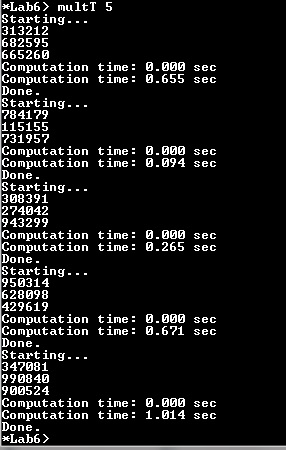
\includegraphics[width= 200px]{snippet}

Where the first computation time is of exM1 and the second one of expM. exM1 is thus significanlty faster.

\section*{Exercise 4}

\lstinputlisting[language=HaskellUlisses, firstline=74, lastline=85]{Lab6.hs}

k = 1, k =2 and k = 3 give 4 as a prime number. When the value of k gets higher there are less fool primes found, this is because more different random numbers are chosen for \emph{a} which lowers the probability a composite number is considered a prime. 

\vspace{0.5cm}
\section*{Exercise 5}

\lstinputlisting[language=HaskellUlisses, firstline=87, lastline=98]{Lab6.hs}

Carmichael numbers almost always pass the Fermat's primality check. That was also shown in the testing, most of the numbers passed our test.
 
The Carmichael numbers are of the form $ b^{n}\equiv b\pmod{n} $ for all integers $1<b<n-1 $. This is also how Fermat's little theorem define prime numbers ( $a^{p-1} \equiv 1 \pmod p.$) . Because Fermat defines prime numbers in the same way Carmichael defines the Carmichael numbers, the carmichael numbers do satisfy the definition of a prime number used in Fermat's primality check. Although the carmichael numbers are not prime numbers but do satisfy Fermat's definition of a prime number, they pass the testing.
\vspace{0.5cm}

\section*{Exercise 6}
\lstinputlisting[language=HaskellUlisses, firstline=99, lastline=110]{Lab6.hs}

Although some Carmichael numbers still pass the Miller-Rabin primality, these are significantly less than with Fermat's primality check. If we higher \emph{k}, meaning that we check with more random \emph{a's} we even find that Miller-Rabin doesn't consider any Carmichael numbers as prime numbers.

\lstinputlisting[language=HaskellUlisses, firstline=111, lastline=120]{Lab6.hs}
\begin{verbatim}
*Lab6> lengthCar 500 10
"500"
\end{verbatim}

\begin{verbatim}
*Lab6>lengthMR 500 10
"0"
\end{verbatim}

\section*{Exercise 7}
\lstinputlisting[language=HaskellUlisses, firstline=122, lastline=140]{Lab6.hs}

The numbers that give True for the first argument in the tuple are indeed known Mersenne numbers as can be found on \url{http://en.wikipedia.org/wiki/Mersenne_prime}.

\section*{Exercise 8}
The function $find2PrimesBitL$ takes as input the bitlength of the prime numbers and the number of the iterations the functions is allowed to perform until it finds two different primes. If the function succeeds returns a tupple with the two different primes else returns $(0,0)$. Firstly, this function chooses a random number from $1$ to $2^{bitlength}-1$ to use it as offset inside the requested range $\{2^{bitlength},...,2^{bitlength+1}-1\}$. The function $findPrimeIn$ is  responsible for finding a prime in the given range by testing numbers with primeMR and $k = 40$. The parameter $k$ was chosen after searching the internet and experimenting with the functions from the previous exercises. If the prime is not found 0 is returned. 
\lstinputlisting[language=HaskellUlisses, firstline=141, lastline=161]{Lab6.hs}


\end{document}